% Created by tikzDevice version 0.10.1 on 2017-05-27 13:39:00
% !TEX encoding = UTF-8 Unicode
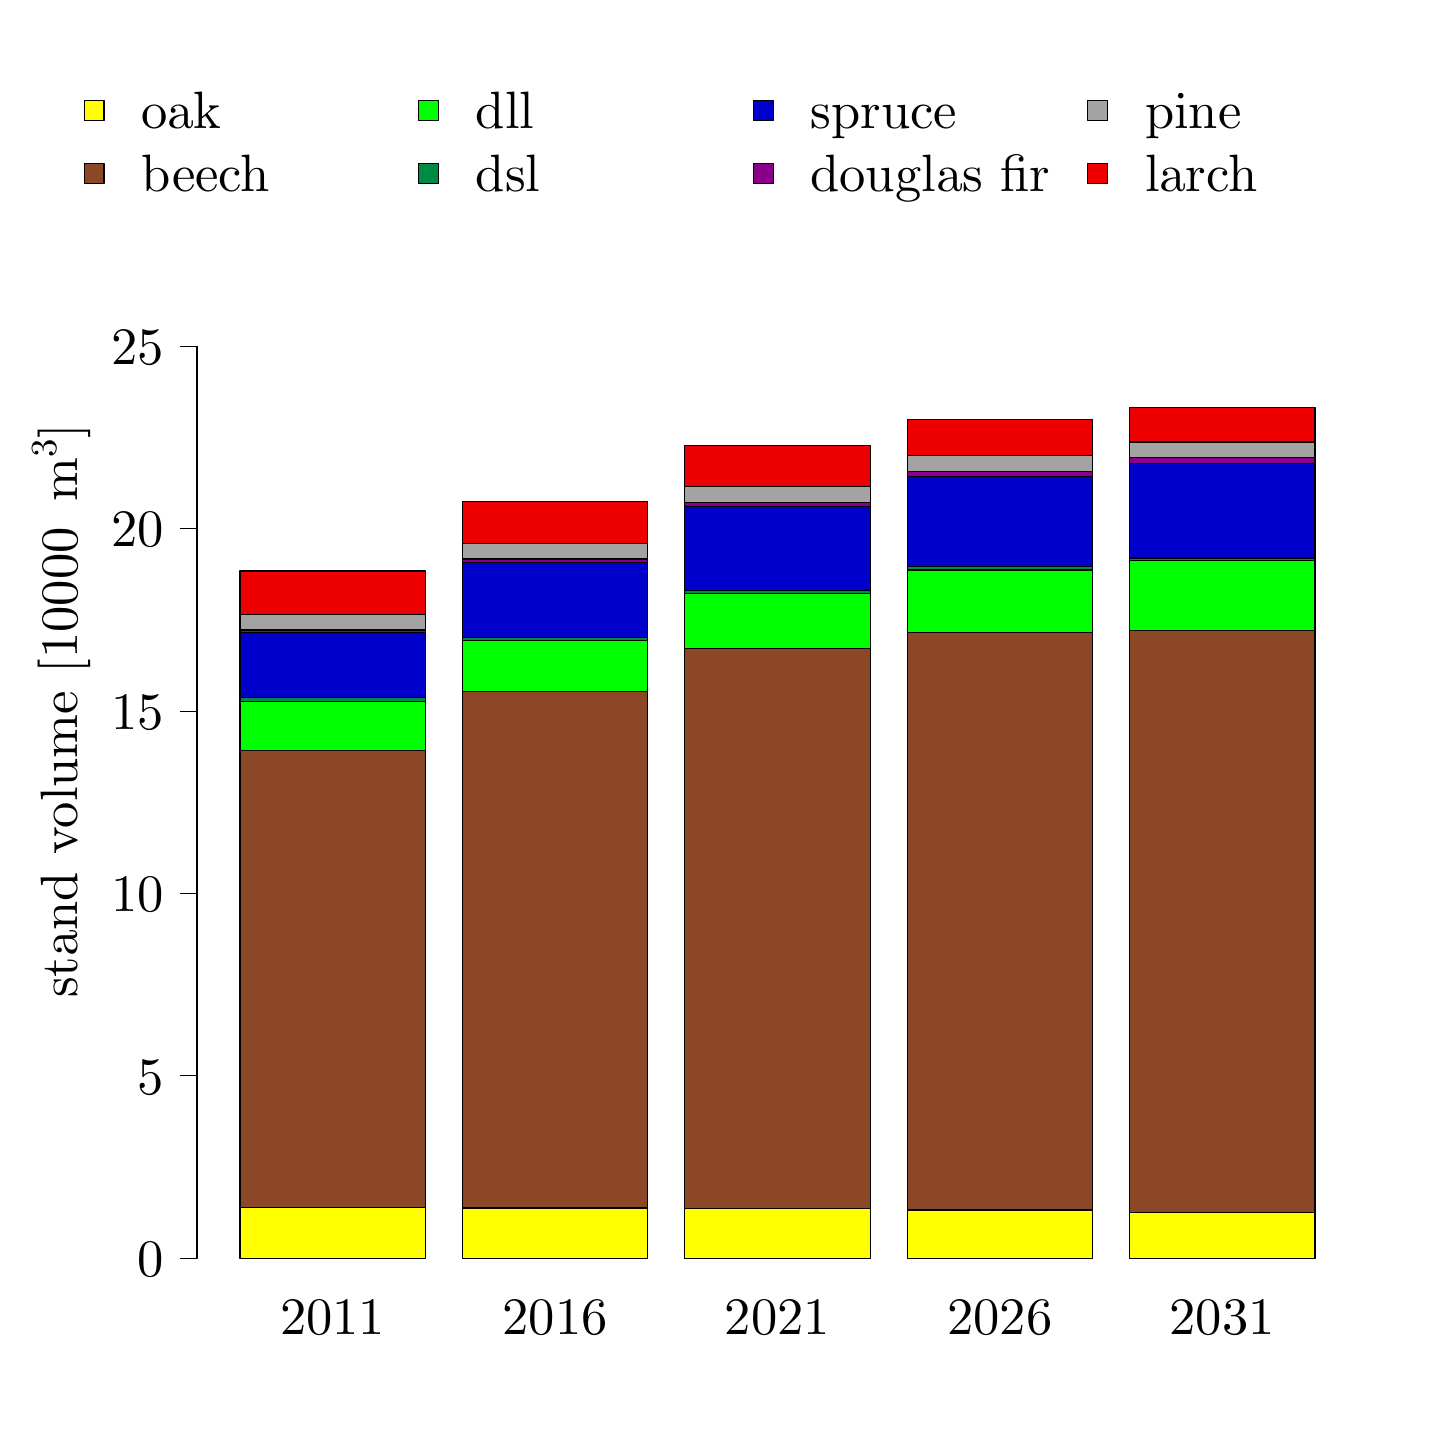
\begin{tikzpicture}[x=1pt,y=1pt]
\definecolor{fillColor}{RGB}{255,255,255}
\path[use as bounding box,fill=fillColor,fill opacity=0.00] (0,0) rectangle (505.89,505.89);
\begin{scope}
\path[clip] (  0.00,  0.00) rectangle (505.89,505.89);
\definecolor{drawColor}{RGB}{0,0,0}
\definecolor{fillColor}{RGB}{255,255,0}

\path[draw=drawColor,line width= 0.4pt,line join=round,line cap=round,fill=fillColor] ( 76.74, 61.20) rectangle (143.71, 79.52);
\definecolor{fillColor}{RGB}{139,71,38}

\path[draw=drawColor,line width= 0.4pt,line join=round,line cap=round,fill=fillColor] ( 76.74, 79.52) rectangle (143.71,244.80);
\definecolor{fillColor}{RGB}{0,255,0}

\path[draw=drawColor,line width= 0.4pt,line join=round,line cap=round,fill=fillColor] ( 76.74,244.80) rectangle (143.71,262.30);
\definecolor{fillColor}{RGB}{0,139,69}

\path[draw=drawColor,line width= 0.4pt,line join=round,line cap=round,fill=fillColor] ( 76.74,262.30) rectangle (143.71,263.78);
\definecolor{fillColor}{RGB}{0,0,205}

\path[draw=drawColor,line width= 0.4pt,line join=round,line cap=round,fill=fillColor] ( 76.74,263.78) rectangle (143.71,287.35);
\definecolor{fillColor}{RGB}{139,0,139}

\path[draw=drawColor,line width= 0.4pt,line join=round,line cap=round,fill=fillColor] ( 76.74,287.35) rectangle (143.71,288.25);
\definecolor{fillColor}{gray}{0.64}

\path[draw=drawColor,line width= 0.4pt,line join=round,line cap=round,fill=fillColor] ( 76.74,288.25) rectangle (143.71,293.71);
\definecolor{fillColor}{RGB}{238,0,0}

\path[draw=drawColor,line width= 0.4pt,line join=round,line cap=round,fill=fillColor] ( 76.74,293.71) rectangle (143.71,309.54);
\definecolor{fillColor}{RGB}{255,255,0}

\path[draw=drawColor,line width= 0.4pt,line join=round,line cap=round,fill=fillColor] (157.10, 61.20) rectangle (224.07, 79.39);
\definecolor{fillColor}{RGB}{139,71,38}

\path[draw=drawColor,line width= 0.4pt,line join=round,line cap=round,fill=fillColor] (157.10, 79.39) rectangle (224.07,266.07);
\definecolor{fillColor}{RGB}{0,255,0}

\path[draw=drawColor,line width= 0.4pt,line join=round,line cap=round,fill=fillColor] (157.10,266.07) rectangle (224.07,284.30);
\definecolor{fillColor}{RGB}{0,139,69}

\path[draw=drawColor,line width= 0.4pt,line join=round,line cap=round,fill=fillColor] (157.10,284.30) rectangle (224.07,285.42);
\definecolor{fillColor}{RGB}{0,0,205}

\path[draw=drawColor,line width= 0.4pt,line join=round,line cap=round,fill=fillColor] (157.10,285.42) rectangle (224.07,312.71);
\definecolor{fillColor}{RGB}{139,0,139}

\path[draw=drawColor,line width= 0.4pt,line join=round,line cap=round,fill=fillColor] (157.10,312.71) rectangle (224.07,313.89);
\definecolor{fillColor}{gray}{0.64}

\path[draw=drawColor,line width= 0.4pt,line join=round,line cap=round,fill=fillColor] (157.10,313.89) rectangle (224.07,319.39);
\definecolor{fillColor}{RGB}{238,0,0}

\path[draw=drawColor,line width= 0.4pt,line join=round,line cap=round,fill=fillColor] (157.10,319.39) rectangle (224.07,334.69);
\definecolor{fillColor}{RGB}{255,255,0}

\path[draw=drawColor,line width= 0.4pt,line join=round,line cap=round,fill=fillColor] (237.46, 61.20) rectangle (304.43, 79.21);
\definecolor{fillColor}{RGB}{139,71,38}

\path[draw=drawColor,line width= 0.4pt,line join=round,line cap=round,fill=fillColor] (237.46, 79.21) rectangle (304.43,281.55);
\definecolor{fillColor}{RGB}{0,255,0}

\path[draw=drawColor,line width= 0.4pt,line join=round,line cap=round,fill=fillColor] (237.46,281.55) rectangle (304.43,301.29);
\definecolor{fillColor}{RGB}{0,139,69}

\path[draw=drawColor,line width= 0.4pt,line join=round,line cap=round,fill=fillColor] (237.46,301.29) rectangle (304.43,302.52);
\definecolor{fillColor}{RGB}{0,0,205}

\path[draw=drawColor,line width= 0.4pt,line join=round,line cap=round,fill=fillColor] (237.46,302.52) rectangle (304.43,332.85);
\definecolor{fillColor}{RGB}{139,0,139}

\path[draw=drawColor,line width= 0.4pt,line join=round,line cap=round,fill=fillColor] (237.46,332.85) rectangle (304.43,334.29);
\definecolor{fillColor}{gray}{0.64}

\path[draw=drawColor,line width= 0.4pt,line join=round,line cap=round,fill=fillColor] (237.46,334.29) rectangle (304.43,340.02);
\definecolor{fillColor}{RGB}{238,0,0}

\path[draw=drawColor,line width= 0.4pt,line join=round,line cap=round,fill=fillColor] (237.46,340.02) rectangle (304.43,354.75);
\definecolor{fillColor}{RGB}{255,255,0}

\path[draw=drawColor,line width= 0.4pt,line join=round,line cap=round,fill=fillColor] (317.82, 61.20) rectangle (384.79, 78.67);
\definecolor{fillColor}{RGB}{139,71,38}

\path[draw=drawColor,line width= 0.4pt,line join=round,line cap=round,fill=fillColor] (317.82, 78.67) rectangle (384.79,287.42);
\definecolor{fillColor}{RGB}{0,255,0}

\path[draw=drawColor,line width= 0.4pt,line join=round,line cap=round,fill=fillColor] (317.82,287.42) rectangle (384.79,309.93);
\definecolor{fillColor}{RGB}{0,139,69}

\path[draw=drawColor,line width= 0.4pt,line join=round,line cap=round,fill=fillColor] (317.82,309.93) rectangle (384.79,311.11);
\definecolor{fillColor}{RGB}{0,0,205}

\path[draw=drawColor,line width= 0.4pt,line join=round,line cap=round,fill=fillColor] (317.82,311.11) rectangle (384.79,343.72);
\definecolor{fillColor}{RGB}{139,0,139}

\path[draw=drawColor,line width= 0.4pt,line join=round,line cap=round,fill=fillColor] (317.82,343.72) rectangle (384.79,345.62);
\definecolor{fillColor}{gray}{0.64}

\path[draw=drawColor,line width= 0.4pt,line join=round,line cap=round,fill=fillColor] (317.82,345.62) rectangle (384.79,351.22);
\definecolor{fillColor}{RGB}{238,0,0}

\path[draw=drawColor,line width= 0.4pt,line join=round,line cap=round,fill=fillColor] (317.82,351.22) rectangle (384.79,364.22);
\definecolor{fillColor}{RGB}{255,255,0}

\path[draw=drawColor,line width= 0.4pt,line join=round,line cap=round,fill=fillColor] (398.18, 61.20) rectangle (465.15, 77.89);
\definecolor{fillColor}{RGB}{139,71,38}

\path[draw=drawColor,line width= 0.4pt,line join=round,line cap=round,fill=fillColor] (398.18, 77.89) rectangle (465.15,288.16);
\definecolor{fillColor}{RGB}{0,255,0}

\path[draw=drawColor,line width= 0.4pt,line join=round,line cap=round,fill=fillColor] (398.18,288.16) rectangle (465.15,313.24);
\definecolor{fillColor}{RGB}{0,139,69}

\path[draw=drawColor,line width= 0.4pt,line join=round,line cap=round,fill=fillColor] (398.18,313.24) rectangle (465.15,314.25);
\definecolor{fillColor}{RGB}{0,0,205}

\path[draw=drawColor,line width= 0.4pt,line join=round,line cap=round,fill=fillColor] (398.18,314.25) rectangle (465.15,348.56);
\definecolor{fillColor}{RGB}{139,0,139}

\path[draw=drawColor,line width= 0.4pt,line join=round,line cap=round,fill=fillColor] (398.18,348.56) rectangle (465.15,350.57);
\definecolor{fillColor}{gray}{0.64}

\path[draw=drawColor,line width= 0.4pt,line join=round,line cap=round,fill=fillColor] (398.18,350.57) rectangle (465.15,356.15);
\definecolor{fillColor}{RGB}{238,0,0}

\path[draw=drawColor,line width= 0.4pt,line join=round,line cap=round,fill=fillColor] (398.18,356.15) rectangle (465.15,368.68);
\end{scope}
\begin{scope}
\path[clip] (  0.00,  0.00) rectangle (505.89,505.89);
\definecolor{drawColor}{RGB}{0,0,0}

\node[text=drawColor,rotate= 90.00,anchor=base west,inner sep=0pt, outer sep=0pt, scale=  1.90] at ( 18.05,155.32) {stand volume [10000};

\node[text=drawColor,rotate= 90.00,anchor=base west,inner sep=0pt, outer sep=0pt, scale=  1.90] at ( 18.05,325.32) { };

\node[text=drawColor,rotate= 90.00,anchor=base west,inner sep=0pt, outer sep=0pt, scale=  1.90] at ( 18.05,334.82) {m};

\node[text=drawColor,rotate= 90.00,anchor=base west,inner sep=0pt, outer sep=0pt, scale=  1.33] at ( 10.28,350.65) {3};

\node[text=drawColor,rotate= 90.00,anchor=base west,inner sep=0pt, outer sep=0pt, scale=  1.90] at ( 18.05,357.30) {]};

\node[text=drawColor,anchor=base,inner sep=0pt, outer sep=0pt, scale=  1.90] at (110.22, 33.60) {2011};

\node[text=drawColor,anchor=base,inner sep=0pt, outer sep=0pt, scale=  1.90] at (190.58, 33.60) {2016};

\node[text=drawColor,anchor=base,inner sep=0pt, outer sep=0pt, scale=  1.90] at (270.94, 33.60) {2021};

\node[text=drawColor,anchor=base,inner sep=0pt, outer sep=0pt, scale=  1.90] at (351.31, 33.60) {2026};

\node[text=drawColor,anchor=base,inner sep=0pt, outer sep=0pt, scale=  1.90] at (431.67, 33.60) {2031};

\path[draw=drawColor,line width= 0.4pt,line join=round,line cap=round] ( 61.20, 61.20) -- ( 61.20,390.78);

\path[draw=drawColor,line width= 0.4pt,line join=round,line cap=round] ( 61.20, 61.20) -- ( 55.20, 61.20);

\path[draw=drawColor,line width= 0.4pt,line join=round,line cap=round] ( 61.20,127.11) -- ( 55.20,127.11);

\path[draw=drawColor,line width= 0.4pt,line join=round,line cap=round] ( 61.20,193.03) -- ( 55.20,193.03);

\path[draw=drawColor,line width= 0.4pt,line join=round,line cap=round] ( 61.20,258.94) -- ( 55.20,258.94);

\path[draw=drawColor,line width= 0.4pt,line join=round,line cap=round] ( 61.20,324.86) -- ( 55.20,324.86);

\path[draw=drawColor,line width= 0.4pt,line join=round,line cap=round] ( 61.20,390.78) -- ( 55.20,390.78);

\node[text=drawColor,anchor=base east,inner sep=0pt, outer sep=0pt, scale=  1.90] at ( 49.20, 54.66) {0};

\node[text=drawColor,anchor=base east,inner sep=0pt, outer sep=0pt, scale=  1.90] at ( 49.20,120.57) {5};

\node[text=drawColor,anchor=base east,inner sep=0pt, outer sep=0pt, scale=  1.90] at ( 49.20,186.49) {10};

\node[text=drawColor,anchor=base east,inner sep=0pt, outer sep=0pt, scale=  1.90] at ( 49.20,252.40) {15};

\node[text=drawColor,anchor=base east,inner sep=0pt, outer sep=0pt, scale=  1.90] at ( 49.20,318.32) {20};

\node[text=drawColor,anchor=base east,inner sep=0pt, outer sep=0pt, scale=  1.90] at ( 49.20,384.23) {25};
\end{scope}
\begin{scope}
\path[clip] (  1.20,  1.20) rectangle (504.69,498.69);
\definecolor{drawColor}{RGB}{0,0,0}
\definecolor{fillColor}{RGB}{255,255,0}

\path[draw=drawColor,line width= 0.4pt,line join=round,line cap=round,fill=fillColor] ( 20.40,472.30) rectangle ( 27.57,479.48);
\definecolor{fillColor}{RGB}{139,71,38}

\path[draw=drawColor,line width= 0.4pt,line join=round,line cap=round,fill=fillColor] ( 20.40,449.50) rectangle ( 27.57,456.68);
\definecolor{fillColor}{RGB}{0,255,0}

\path[draw=drawColor,line width= 0.4pt,line join=round,line cap=round,fill=fillColor] (141.29,472.30) rectangle (148.47,479.48);
\definecolor{fillColor}{RGB}{0,139,69}

\path[draw=drawColor,line width= 0.4pt,line join=round,line cap=round,fill=fillColor] (141.29,449.50) rectangle (148.47,456.68);
\definecolor{fillColor}{RGB}{0,0,205}

\path[draw=drawColor,line width= 0.4pt,line join=round,line cap=round,fill=fillColor] (262.18,472.30) rectangle (269.36,479.48);
\definecolor{fillColor}{RGB}{139,0,139}

\path[draw=drawColor,line width= 0.4pt,line join=round,line cap=round,fill=fillColor] (262.18,449.50) rectangle (269.36,456.68);
\definecolor{fillColor}{gray}{0.64}

\path[draw=drawColor,line width= 0.4pt,line join=round,line cap=round,fill=fillColor] (383.07,472.30) rectangle (390.25,479.48);
\definecolor{fillColor}{RGB}{238,0,0}

\path[draw=drawColor,line width= 0.4pt,line join=round,line cap=round,fill=fillColor] (383.07,449.50) rectangle (390.25,456.68);

\node[text=drawColor,anchor=base west,inner sep=0pt, outer sep=0pt, scale=  1.90] at ( 41.09,469.35) {oak};

\node[text=drawColor,anchor=base west,inner sep=0pt, outer sep=0pt, scale=  1.90] at ( 41.09,446.55) {beech};

\node[text=drawColor,anchor=base west,inner sep=0pt, outer sep=0pt, scale=  1.90] at (161.98,469.35) {dll};

\node[text=drawColor,anchor=base west,inner sep=0pt, outer sep=0pt, scale=  1.90] at (161.98,446.55) {dsl};

\node[text=drawColor,anchor=base west,inner sep=0pt, outer sep=0pt, scale=  1.90] at (282.87,469.35) {spruce};

\node[text=drawColor,anchor=base west,inner sep=0pt, outer sep=0pt, scale=  1.90] at (282.87,446.55) {douglas fir};

\node[text=drawColor,anchor=base west,inner sep=0pt, outer sep=0pt, scale=  1.90] at (403.76,469.35) {pine};

\node[text=drawColor,anchor=base west,inner sep=0pt, outer sep=0pt, scale=  1.90] at (403.76,446.55) {larch};
\end{scope}
\end{tikzpicture}
